\documentclass[conference]{IEEEtran}

% ========= 日本語対応(LuaLaTeX推奨) =========
\usepackage{luatexja}
\usepackage{luatexja-fontspec}
\setmainjfont{HaranoAjiMincho}
\setsansjfont{HaranoAjiGothic}

% ========= 一般パッケージ =========
\usepackage{amsmath,amssymb}
\usepackage{graphicx}
\usepackage{booktabs}
\usepackage{array}
\usepackage{url}
\usepackage[hidelinks]{hyperref}
\usepackage{cite}

% ========= 図・グラフ(TikZ/PGFPlots)=========
\usepackage{tikz}
\usetikzlibrary{arrows.meta,decorations.pathreplacing,calc,patterns}
\usepackage{pgfplots}
\pgfplotsset{compat=1.17}

% ========= タイトル =========
\title{DRAM技術導入とその戦略的位置づけ(1997--2001)\\
\large 酒田FabにおけるDRAM/PSRAMとロジック展開の関連}

% ========= 著者情報 =========
\author{%
  \IEEEauthorblockN{三溝 真一 (Shinichi Samizo)}%
  \IEEEauthorblockA{独立系半導体研究者(元セイコーエプソン)\\%
  Independent Semiconductor Researcher (ex-Seiko Epson)\\%
  Email: \href{mailto:shin3t72@gmail.com}{shin3t72@gmail.com}\\%
  GitHub: \url{https://github.com/Samizo-AITL}}%
}

\begin{document}
\maketitle

\begin{abstract}
\textbf{(日本語)}\\
本論文は,1997--2001年に酒田Fabが三菱電機からの技術移管を通じて
\mbox{0.5\,$\mu$m} $\rightarrow$ \mbox{0.35\,$\mu$m} $\rightarrow$ \mbox{0.25\,$\mu$m} の
DRAMプロセスを短期間で習得し,得られた知見を先端ロジックおよび高耐圧混載CMOSへ展開して
液晶ドライバー製品化へ結びつけた過程を,筆者の実体験に基づき整理する。
主要な不良モード(Pause/Disturb Refresh)の物理起源と対策,量産歩留まりの推移を示し,
獲得知見の活用と限界を考察する。\\[1ex]

\textbf{(English)}\\
We review 1997--2001 when Epson Sakata Fab assimilated DRAM processes
(0.5\,\textmu m $\rightarrow$ 0.35\,\textmu m $\rightarrow$ 0.25\,\textmu m) transferred from Mitsubishi.
The DRAM know-how was extended to advanced logic and high-voltage mixed CMOS, enabling LCD driver products.
Key failure modes, countermeasures, and yield evolution are summarized.
\end{abstract}

\begin{IEEEkeywords}
DRAM, VSRAM/PSRAM, 0.25\,$\mu$m, retention failure, disturb failure, Sakata Fab, technology transfer, high-voltage mixed CMOS, LCD driver
\end{IEEEkeywords}

\section{序論}
1997年,当時の半導体産業は \textit{Windows~95} の普及と Pentium~II の登場を契機に急伸した。
製造技術では 8インチウェーハラインと 0.35\,\textmu m 世代の量産が進み,DRAM とロジックの国際競争が激化した。
酒田FabはDRAMを「目的」ではなく「先端プロセス自前化の手段」と位置づけ,最終的にロジック/高耐圧混載CMOS(液晶ドライバー)へ接続する戦略を採った。
本稿は,その立ち上げ・不良解析・歩留まり改善・展開と限界を,筆者の実務経験に基づき記述する。

\section{第1章:0.5\,\texorpdfstring{$\mu$m}{μm} と 0.35\,\texorpdfstring{$\mu$m}{μm} 世代の立ち上げ}
\subsection{0.5\,\textmu m 16M DRAM}
熊本Fabで確立されたプロセスを忠実移管。設備親和性が高く,初期から安定歩留まりで短期間に量産へ到達した。

\subsection{0.35\,\textmu m 64M DRAM:洗浄フロー差異と「鏡写し」}
1997年秋,試作30ロット超で形状不良が続発。原因は\emph{洗浄フロー差異}(熊本:硫酸過水→アンモニア過水→塩酸過水/酒田:硫酸過水を省略)。
表面状態差が後工程プラズマと相互作用して膜厚ばらつきを拡大させた。
\textbf{解決策}は熊本プロセスの\emph{完全鏡写し}(フロー・装置条件・手順を省略なく再現)で,形状不良は終息し量産化に成功した。

\subsection*{小括}
0.5\,\textmu m:忠実移管で早期安定化。\quad
0.35\,\textmu m:洗浄差による不良を\emph{鏡写し}で解消し,次世代への足場を構築。

\section{第2章:0.25\,\texorpdfstring{$\mu$m}{μm} 世代64M DRAMの立ち上げ}

\subsection{SCF方式と初期歩留まり}
1998年,次世代 0.25\,\textmu m 64M DRAM の立ち上げに着手。
本プロジェクトでも三菱の \emph{Short Cycle Feedback (SCF)} を継続採用(SCF自体は 0.5\,\textmu m 期から運用)。
短サイクルで形状・電気を評価→条件修正→再評価を繰り返し,\textbf{初期本番で約65\%}を確保。
代表手順:移管条件の流動票展開/各要所で形式ロット途中止め・SEM確認/本番ロットで長期信頼性評価。

\subsection{保持時間モデルと不良モード解析}
初期不良は \emph{Pause Refresh Fail} に集中。32\,ms→64\,ms→128\,ms と停止時間を延長すると単ビットがランダム散発。
ライン欠陥やエッジ集中は無く,全域ランダム分布(Fig.~\ref{fig:failmap})。
保持時間は
\begin{equation}
\tau=\frac{C_{\mathrm{cell}} \cdot V_{\mathrm{cell}}}{I_{\mathrm{leak}}}
\end{equation}
で表され,$C_{\mathrm{cell}}$ と $V_{\mathrm{cell}}$ は設計通りで,支配因子はリーク $I_{\mathrm{leak}}$。
解析の結果,キャパシタ誘電体欠陥は否定され,\textbf{拡散層ジャンクションリーク}が主因と特定。
同一座標での再現性から系統的(プロセス起因)と判断した(Fig.~\ref{fig:dram_cross_section})。

\begin{figure}[t]
\centering
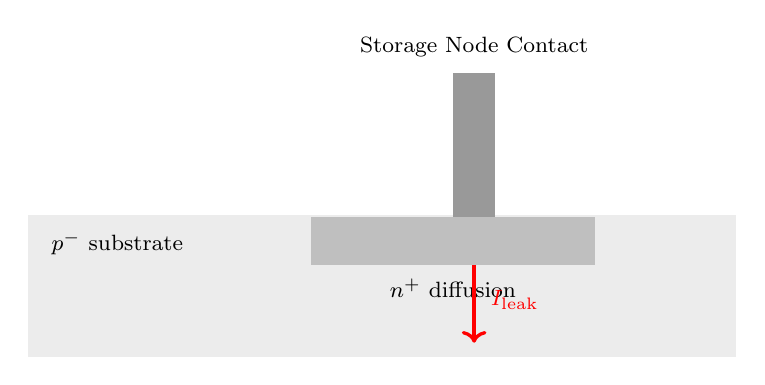
\begin{tikzpicture}[scale=1.8]
  % p- substrate
  \fill[gray!15] (-1,0) rectangle (4,-1.0);
  \node[anchor=north west] at (-0.9,-0.05) {\footnotesize $p^-$ substrate};
  % n+ diffusion
  \fill[gray!50] (1,-0.01) rectangle (3,-0.35);
  \node[anchor=north] at (2,-0.38) {\footnotesize $n^+$ diffusion};
  % Storage node contact (filled, no border)
  \fill[black!40] (2,-0.01) rectangle (2.3,1.0);
  \node[anchor=south] at (2.15,1.05) {\footnotesize Storage Node Contact};
  % Leakage arrow
  \draw[->,very thick,red] (2.15,-0.35) -- (2.15,-0.9);
  \node[anchor=west,red] at (2.2,-0.6) {\footnotesize $I_{\mathrm{leak}}$};
\end{tikzpicture}
\caption{DRAM セル断面の概念図(SNコンタクト/$n^+$拡散層/$p^-$基板)。赤矢印は $n^+\!\to\!p^-$ のジャンクションリーク $I_{\mathrm{leak}}$。}
\label{fig:dram_cross_section}
\end{figure}

\begin{figure}[t]
\centering
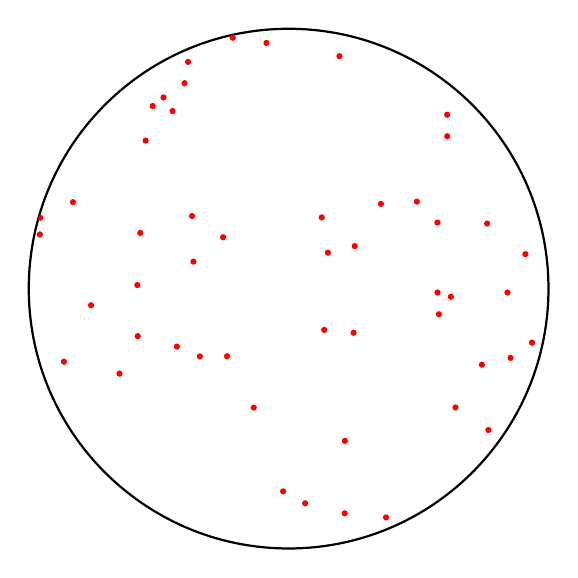
\begin{tikzpicture}[scale=0.22]
  \def\R{15}
  \draw[thick] (0,0) circle (\R);
  \begin{scope}
    \clip (0,0) circle (\R);
    \foreach \i in {1,...,60}{
      \pgfmathsetmacro{\xx}{(rnd*2-1)*\R}
      \pgfmathsetmacro{\yy}{(rnd*2-1)*\R}
      \fill[red] (\xx,\yy) circle (0.18);
    }
  \end{scope}
\end{tikzpicture}
\caption{Pause Refresh Fail のフェイルビットマップ例(ウエハ外周円+ランダム散点)。}
\label{fig:failmap}
\end{figure}

\subsection{プラズマダメージ仮説}
ジャンクションリーク増大の駆動因子として \emph{プラズマダメージ} を特定。
感受性の高い「ゲートエッチ後の酸化膜露出」「LDD工程の繰返しアッシング」により界面欠陥準位が生成し,
熱励起キャリア生成を介してリークが増大したと推定。

\subsection{対策と効果}
根本対策は,\textbf{レジスト剥離を O$_2$アッシングから \emph{硫酸剥離} へ全面切替}すること。
感受性工程後のプラズマ曝露をゼロ化し,界面欠陥生成を根本抑制した
(アッシングの低パワー化は行わず,\emph{フロー自体を変更})。

\begin{table}[t]
  \centering
  \caption{レジスト剥離フローの切替(Before/After)}
  \label{tab:resist_flow}
  \footnotesize
  \begin{tabular}{p{0.25\linewidth} p{0.65\linewidth}}
    \toprule
    従来(Before) & O$_2$アッシングによるドライ剥離 \\
    対策後(After) & \textbf{硫酸剥離} によるウエット剥離 \\
    主効果 & プラズマ曝露ゼロ化,界面欠陥・ジャンクションリーク抑制 \\
    歩留まり & 65\% $\rightarrow$ 80\%台後半(Pause 改善が支配) \\
    \bottomrule
  \end{tabular}
\end{table}

この切替により Pause 不良は大幅減少し,\textbf{量産歩留まりは 65\%→80\%台後半}へ改善した(Fig.~\ref{fig:yield_trend})。

\begin{figure}[t]
\centering
\begin{tikzpicture}
\begin{axis}[
  width=\linewidth,height=6cm,ymin=0,ymax=100,grid=both,
  ylabel={歩留まり(\%)},xlabel={プロセス世代},
  symbolic x coords={0.5\,\mu m,0.35\,\mu m,0.25\,\mu m,VSRAM},
  xtick=data,xticklabel style={align=center},
  legend style={at={(0.5,-0.28)},anchor=north,draw=none,fill=none,font=\footnotesize},
  legend columns=2,clip=false
]
  \addplot+[semithick,mark=*]
    coordinates {(0.5\,\mu m,95) (0.35\,\mu m,20) (0.25\,\mu m,65) (VSRAM,30)};
  \addlegendentry{初期}
  \addplot+[semithick,mark=square*]
    coordinates {(0.5\,\mu m,95) (0.35\,\mu m,86) (0.25\,\mu m,88) (VSRAM,80)};
  \addlegendentry{改善後}
\end{axis}
\end{tikzpicture}
\caption{酒田Fabにおける世代別歩留まり推移(1カラム収まり)。}
\label{fig:yield_trend}
\end{figure}

\subsection*{小括}
SCFにより迅速に条件整備し初期65\%を確保。主因はジャンクションリークで,\textbf{硫酸剥離への全面切替}により 80\%台後半へ改善。
表面処理とプラズマ影響の管理が最重要であることをFab標準知見として確立。

% ============== 第3章 ==============
\section{第3章:VSRAM(2001年)— Pause/Disturb対策と歩留まり改善}

\subsection{開発背景と初期状況}
2001年,\emph{0.25\,\textmu m DRAMプロセス流用+内部リフレッシュ制御}でVSRAM(疑似SRAM)を量産化。
モバイル仕様(低消費/90$^\circ$C保証)のため初期歩留まりは \textbf{30\%} と厳しかった。

\subsection{物理的要因}
Pause は\textbf{ジャンクションリーク加速}が主因。温度上昇で指数的に悪化し,$V_{bs}$ 強化で抑制可能(Fig.~\ref{fig:pause_temp_junc})。
Disturb は\textbf{短チャネル効果(SCE)}によるオフリーク増大と隣接セル誤反転が主因で,温度上昇でさらに顕著(Fig.~\ref{fig:disturb_temp_sce})。

\begin{figure}[t]
\centering
\begin{tikzpicture}
\begin{axis}[
  width=\linewidth,height=6cm,ymode=log,ymin=1e-2,ymax=1e2,
  xmin=25,xmax=100,xtick={25,40,60,80,90,100},
  grid=both, xlabel={温度 [$^\circ$C]}, ylabel={ジャンクションリーク $I_{\mathrm{junc}}$(相対)},
  legend style={at={(0.5,-0.22)},anchor=north,draw=none,fill=none}, clip=false
]
  \addplot+[semithick,mark=*] coordinates {(25,0.02) (40,0.06) (60,0.3) (80,1.6) (90,3.2) (100,6.0)};
  \addlegendentry{$V_{bs}=-1$\,V}
  \addplot+[semithick,mark=square*] coordinates {(25,0.01) (40,0.03) (60,0.12) (80,0.45) (90,0.9) (100,1.8)};
  \addlegendentry{$V_{bs}=-3$\,V}
\end{axis}
\end{tikzpicture}
\caption{Pause:温度上昇で $I_{\mathrm{junc}}$ は指数増大。$V_{bs}$ 強化で抑制可。}
\label{fig:pause_temp_junc}
\end{figure}

\begin{figure}[t]
\centering
\begin{tikzpicture}
\begin{axis}[
  width=\linewidth,height=6cm,ymode=log,ymin=1e-3,ymax=1e1,
  xmin=25,xmax=100,xtick={25,40,60,80,90,100},
  grid=both, xlabel={温度 [$^\circ$C]}, ylabel={トランジスタリーク $I_{\mathrm{off}}$(相対)},
  legend style={at={(0.5,-0.22)},anchor=north,draw=none,fill=none}, clip=false
]
  \addplot+[semithick,mark=triangle*] coordinates {(25,0.004) (40,0.01) (60,0.05) (80,0.22) (90,0.45) (100,0.9)};
  \addlegendentry{CD=0.25\,\textmu m}
  \addplot+[semithick,mark=*] coordinates {(25,0.01) (40,0.03) (60,0.15) (80,0.7) (90,1.4) (100,2.8)};
  \addlegendentry{CD=0.20\,\textmu m}
\end{axis}
\end{tikzpicture}
\caption{Disturb:短チャネル化で $I_{\mathrm{off}}$ 増大。温度上昇で指数加速。}
\label{fig:disturb_temp_sce}
\end{figure}

\subsection{対策と実装}
\begin{itemize}
  \item \textbf{Pause対策}:HF洗浄回数の最小化(ゲート酸化膜残膜確保),\;$V_{bs}$ 強化($-1$V$\to-3$V)でジャンクションリーク抑制。
  \item \textbf{Disturb対策}:ゲートCD中心の厳密管理,\;$V_{bs}$ 強化で $V_{th}$ 上昇,\;セルの\emph{チャネルドーピングを許容範囲で増加}し $V_{th}$ を押し上げて誤反転耐性を向上。
\end{itemize}

\begin{table}[t]
\centering
\caption{Pause / Disturb 不良に対する主因と主な対策(1カラム収まり)}
\label{tab:countermeasures}
\footnotesize
\begin{tabular}{p{0.18\linewidth} p{0.28\linewidth} p{0.46\linewidth}}
\toprule
不良モード & 主因 & 主な対策 \\
\midrule
Pause   & ジャンクションリーク & HF洗浄制御,$V_{bs}$強化 \\
Disturb & 短チャネル効果       & CD管理,チャネルドーピング,$V_{bs}$強化 \\
\bottomrule
\end{tabular}
\end{table}

\subsection{効果と歩留まり推移}
対策により,Pause/Disturb はともに高温条件で顕著に改善。\;
\textbf{歩留まりは 30\% $\to$ 80\%台}に回復し量産水準へ到達。

\section{第4章:0.18\,\texorpdfstring{$\mu$m}{μm} トレンチ系の評価と断念}

\subsection{評価対象と背景}
VSRAMの後継候補として,NANYA 0.18\,\textmu m(東芝系)トレンチDRAMプロセスを用いた試作評価を実施。
狙いは高密度・低消費の両立。

\subsection{技術的特徴とボトルネック}
トレンチは面積効率に優れる一方でジャンクション面積が増大し,\textbf{高温リークが支配的}になりやすい。
標準DRAMの 80$^\circ$C は満たすが,\textbf{モバイル必須の 90$^\circ$C 保証}では設計余裕が乏しい。

\subsection{課題の顕在化}
90$^\circ$C 条件で Pause/Disturb の顕在化,高温リークの顕著な増加を確認。
Fig.~\ref{fig:trench_area_leak} の通り,\textbf{ジャンクション面積にほぼ比例}して $I_{\mathrm{junc}}$ が増加し,高温ほど傾きが大きい。

\begin{figure}[t]
\centering
\begin{tikzpicture}
\begin{axis}[
  width=\linewidth,height=6cm,
  xlabel={ジャンクション面積(相対)}, ylabel={ジャンクションリーク $I_{\mathrm{junc}}$(相対)},
  xmin=0.5,xmax=2.5,ymin=0,ymax=3.5,xtick={0.5,1.0,1.5,2.0,2.5},
  grid=both,legend style={at={(0.5,-0.22)},anchor=north,draw=none,fill=none},clip=false
]
  \addplot+[semithick,mark=square*] coordinates {(0.5,0.25) (1.0,0.5) (1.5,0.8) (2.0,1.1) (2.5,1.4)};
  \addlegendentry{80$^\circ$C}
  \addplot+[semithick,mark=*] coordinates {(0.5,0.5) (1.0,1.0) (1.5,1.6) (2.0,2.2) (2.5,2.9)};
  \addlegendentry{90$^\circ$C}
\end{axis}
\end{tikzpicture}
\caption{トレンチキャパ:面積とともに $I_{\mathrm{junc}}$ が増加。高温(90$^\circ$C)で増加率が大。}
\label{fig:trench_area_leak}
\end{figure}

\subsection{評価結果と戦略判断}
NANYA 0.18\,\textmu m トレンチでは 90$^\circ$C 動作保証の達成が困難と判断し,次世代VSRAMは\textbf{断念}。
同時に,酒田の主戦場を\textbf{高耐圧混載CMOS(液晶ドライバー)}へ集中させる戦略へ明確にシフト。

\section{結論}
1997--2001年の酒田FabにおけるDRAM導入は「事業の最終目的」ではなく\textbf{先端プロセス自前化の手段}であった。
0.5/0.35\,\textmu m での忠実移管と\emph{鏡写し},0.25\,\textmu m での SCF と不良解析を通じ,
\textbf{硫酸剥離への全面切替}などの実践知見を確立。
VSRAMではモバイル仕様特有の Pause/Disturb を対策し歩留まりを 30\%→80\%台に改善。
一方で 0.18\,\textmu m トレンチは高温保持の壁により断念。
結果として獲得知見は\textbf{高耐圧混載CMOS}(液晶ドライバー)に直結し,事業の中核競争力を形成した。

\section*{参考文献}
\begin{thebibliography}{00}
\bibitem{sze2006psd}
S.~M.~Sze and K.~K.~Ng, \emph{Physics of Semiconductor Devices}, 3rd ed., Wiley, 2006.

\bibitem{tanaka1996dramtrends}
T.~Tanaka et al., ``Trends and Challenges in DRAM Scaling,'' \emph{IEEE J. Solid-State Circuits}, 31(11), pp.~1615--1624, 1996.

\bibitem{rizzoli2000retention}
L.~Rizzoli et al., ``Retention and Disturb Characterization in 0.25\,\textmu m DRAM,'' in \emph{Proc. International Test Conference}, 2000.

\bibitem{okhonin1998retention}
S.~Okhonin et al., ``Retention Time and Junction Leakage in Deep Submicron DRAM,'' in \emph{IEDM Tech. Dig.}, pp.~549--552, 1998.

\bibitem{wong1999dram}
H.-S.~P.~Wong, ``Technology and Device Scaling for DRAM,'' \emph{IBM J. Res. Dev.}, 43(1–2), pp.~133--168, 1999.

\bibitem{chang1994plasma}
C.~Chang and S.~C.~Lee, ``Plasma-Induced Damage on Gate Oxides,'' \emph{J. Electrochem. Soc.}, 141(9), pp.~2512--2517, 1994.

\bibitem{mosys2001}
MoSys Inc., ``1T-SRAM Technology Overview,'' White Paper, 2001.

\bibitem{kim2002psram}
J.~Kim et al., ``Low Power Refresh Schemes for Mobile DRAM/PSRAM,'' in \emph{Symp. VLSI Circuits}, pp.~190--193, 2002.

\bibitem{schuegraf1997plasma}
K.~Schuegraf et al., ``Impact of Plasma Damage on Junction Leakage and Gate Oxide Reliability,'' in \emph{VMIC Proc.}, pp.~73--79, 1997.
\end{thebibliography}

\section*{著者略歴}
\noindent\textbf{三溝 真一 (Shinichi Samizo)}:
信州大学大学院 工学系研究科 電気電子工学専攻 修士。
セイコーエプソンで半導体ロジック/メモリ/高耐圧インテグレーション,
およびインクジェット薄膜ピエゾ・PrecisionCore プリントヘッド製品化に従事。
現在は独立系半導体研究者として,プロセス/デバイス教育,メモリアーキテクチャ,
AIシステム統合などに取り組む。連絡先:\href{mailto:shin3t72@gmail.com}{shin3t72@gmail.com}

\end{document}





